\subsection{Application des conditions de Stoney}

\begin{frame}
    \frametitle{Dépôt d'aluminium sur un substrat de silicium}
    On étudie ici
les contraintes qui se développent dans un film d’aluminium d’1 µm d’épaisseur déposé sur un substrat
de silicium de 500 µm d’épaisseur.
    \begin{itemize}
        \item Le dépôt s’effectue à une température de 50$^{\circ}C$
        \item A la fin du dépôt, le substrat et le film sont supposés être dans leur état naturel.
        \item le composant est un disque parfait de rayon égal à 200mm.
        \item Il est ensuite refroidi jusqu’à la température ambiante de 20$^{\circ}C$.
    \end{itemize}
\end{frame}

\begin{frame}
    \frametitle{Calcul de la courbure et des contraintes}
    Les hypothèses de Stoney sont remplies:
    $$\frac{h_{f}}{h_{s}} = 2.10^{-3},   ~ ~ ~ \frac{M_{f}h_{f}}{M_{s}h_{s}} = 1,1.10^{-3}$$
    On peut donc appliquer la formule de Stoney pour déterminer la courbure du bilame :
    $$c = 8,3.10^{-3} m^{-1} ~ et ~ R = \frac{1}{c}=120m$$
    \begin{figure}
        \centering
        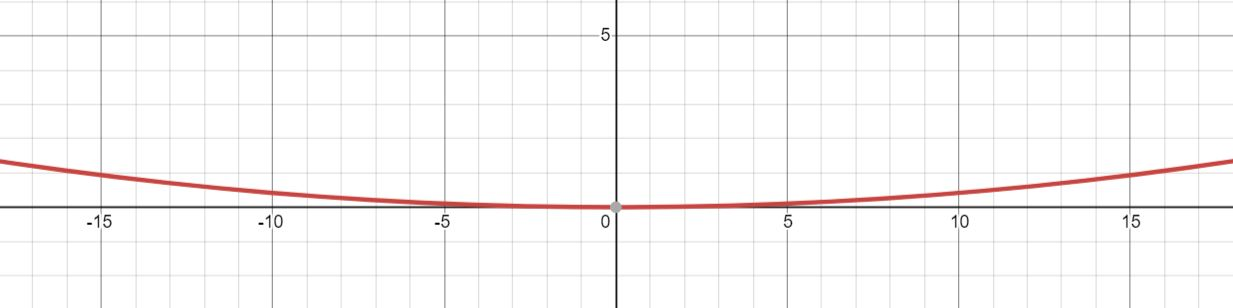
\includegraphics[scale=0.4]{imgs/courbure positive.JPG}
    \end{figure}
\end{frame}

\begin{frame}
    \frametitle{Calcul de la courbure et des contraintes}
    L'expression de la courbure permet d'accéder à une estimation de la contrainte moyenne dans le film : 
    $$ \sigma_{11}^{f} = \frac{M_sh_s^2}{6h_f}\cdot c $$
    Donc:
    $$ \sigma_{11}^{f} = 63 MPa ~~~ et ~~~ \sigma_{11}^{s} = -0.13 MPa $$ 
\end{frame}

\begin{frame}
    \frametitle{Méthodes de mesure de la courbure}
    \textbf{\Large{Méthode mécanique (Profilomètre)}}
    \begin{itemize}
        \item Le but c'est d'enregistrer le déplacement $u_3$ et d'en déduire la courbure
    \end{itemize}
    \begin{figure}
        \centering
        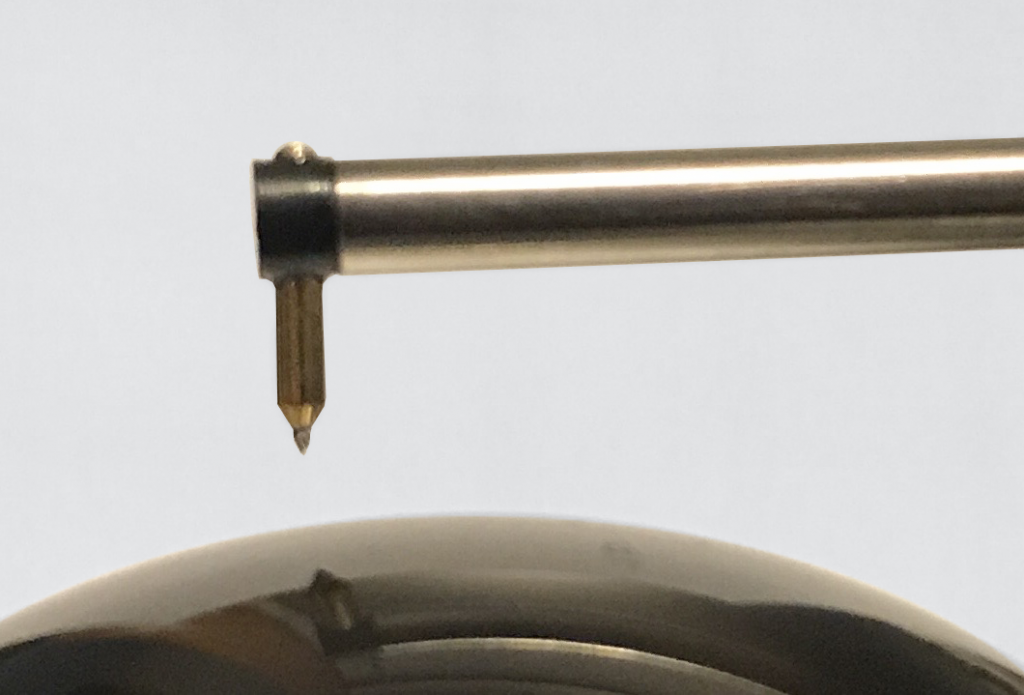
\includegraphics[scale=0.2]{imgs/Digital_Metrology-Measuring_Arcs_with_Stylus_1_Stylus_on_Ball-1024x695.png}
    \end{figure}
\end{frame}

\begin{frame}
    \frametitle{Méthodes de mesure de la courbure}
    \textbf{\Large{Méthode de diffraction X-Ray}}
    \begin{figure}
        \centering
        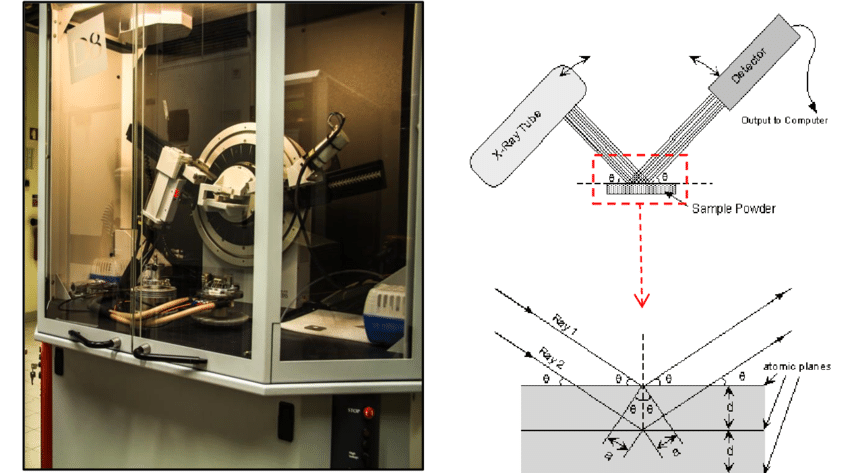
\includegraphics[scale=0.3]{imgs/XRD-equipment-and-schematic-of-X-ray-diffraction-adopted-from-Erdem-2012-Nelson-2015.png}
    \end{figure}
\end{frame}

\begin{frame}
    \frametitle{Méthodes de mesure de la courbure}
    \begin{itemize}
        \item Cette méthode détermine successivement l'angle de Bragg pour l'intensité de diffraction maximale à différents emplacements radiaux de la surface du substrat.
        \item Le rayon de courbure du substrat est la distance radiale entre les deux endroits de la surface où sont effectuées les mesures de diffraction, divisée par la différence des positions angulaires des maxima d'intensités.
    \end{itemize}
    $$R = \frac{1}{c} = \frac{r_2-r_1}{\theta _2-\theta_1}$$
\end{frame}

\begin{frame}
    \frametitle{Méthodes de mesure de la courbure}
    \textbf{\Large{Méthode optique}}
    \begin{itemize}
        \item Un faisceau laser incident sur la surface du substrat est balayé le long d'une ligne droite.
        \item La déviation angulaire 2$\theta$ du faisceau réfléchi par rapport à l'incident est mesurée en fonction de la distance $r$ par rapport à un point de référence.
        \item La déviation du faisceau balayé est surveillée par un détecteur sensible à la position.
        \item La courbure est liée à l'angle $\theta$ qui dépend de $r$.
    \end{itemize}
    \begin{figure}
        \centering
        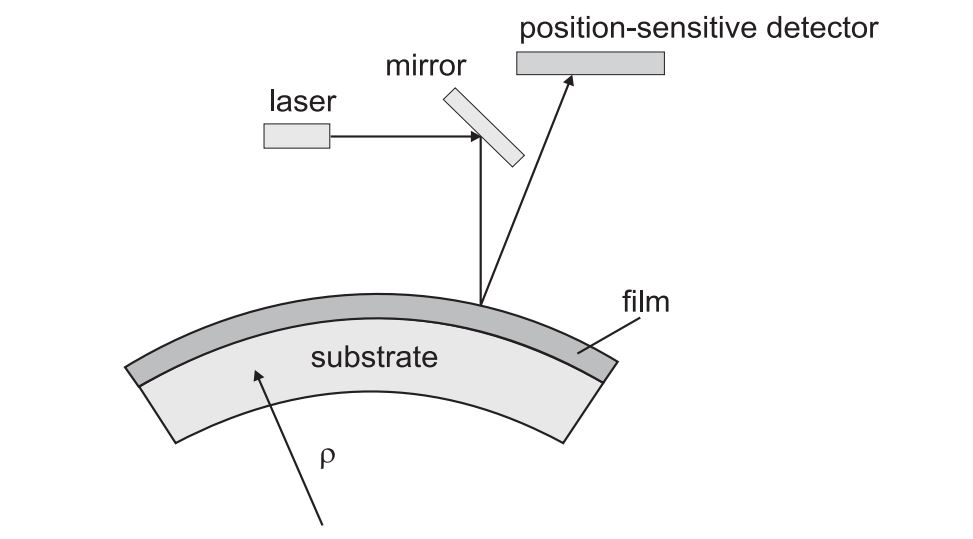
\includegraphics[scale=0.3]{imgs/laser method.JPG}
    \end{figure}
\end{frame}

\begin{frame}
    \frametitle{Contraintes d'épitaxie}
    \textbf{\Large{C'est quoi l'épitaxie ?}}
    \begin{itemize}
        \item C'est une technique de croissance orientée, de 2 cristaux possédant un certain nombre d'éléments de symétrie communs dans leurs réseaux cristallins.
        \item Elle est utilisée pour faire croître des couches minces, de quelques nanomètres d'épaisseur. Pour cela, des atomes sont déposés sur la surface parfaitement polie d'un monocristal, le substrat.
        \item Le substat est choisi de façon à avoir des paramètres de maille proches de ceux du cristal qui souhaite être obtenu.
    \end{itemize}
    Il y a deux types d'épitaxie:
    \begin{itemize}
        \item homoépitaxie   : les 2 matériaux sont identiques.
        \item hétéroépitaxie : les 2 matériaux sont différents.
    \end{itemize}
    Dans le 2ème type, la croissance n'est possible que s'il y a accord de maille, c'est-à-dire qu'il aient le même réseau cristallin et que les paramètres de maille soient assez voisins.
    
\end{frame}

\begin{frame}{Contraintes d'épitaxie}
    \begin{itemize}
        \item La différence des paramètres de maille induit une contrainte dans le plan de base.
        \item Le film se déforme pour avoir le même paramètre de maille que le substrat, donc il n'y a pas de déformation ni de contrainte dans le substrat.$$ \varepsilon _{11} ^{\star s} = 0 $$
        \item Toutefois, ceci n'est pas réaliste puisque aucune contrainte dans le substrat n'équilibre la contrainte dans le film. $\Rightarrow$ Il faut introduire un modèle élastique multicouche pour décrire les déformations présentes lors de la croissance du film sur le substrat.
    \end{itemize}
\end{frame}

\begin{frame}{Contraintes d'épitaxie}
    \begin{itemize}
        \item Ici on prend le cas par exemple des dépôts de silicium–germanium sur un substrat de silicium monocristallin.
        \item le paramètre cristallin $a_{SiGe} = 0.5476$nm du silicium–germanium (pour 80$\%$ de silicium et 20$\%$ de germanium dans le composé binaire) est légèrement plus grand que le paramètre du silicium $a_{Si} = 0.5431$nm en raison de l’implantation des atomes de germanium.
        \item Si le film n’était pas contraint de croître en épitaxie avec le substrat, il se déformerait librement de la quantité:
        $$\varepsilon _{11} ^{\star f} = \varepsilon _{22} ^{\star f} = \varepsilon _{33} ^{\star f} = \frac{a_{SiGe}-a_{Si}}{a_{Si}}  $$
        \item La déformation totale dans le film est donc la somme d’une déformation élastique et de la déformation libre d’épitaxie :
        $$\varepsilon _{11} ^{f} = \varepsilon _{11} ^{ef} + \varepsilon _{11} ^{\star f}$$
    \end{itemize}
\end{frame}

\begin{frame}{Contraintes d'épitaxie}
    \begin{itemize}
        \item Données : $M_f$ = 170 GPa , $h_f$ = 100 nm , $h_s$ = 1 mm
        \item La déformation libre d’épitaxie s’apparente à la dilatation thermique et l’on a l’analogie suivante :
        $$\frac{a_{SiGe}-a_{Si}}{a_{Si}} \equiv \alpha _f(T-T_0) ~~ et ~~ 0 \equiv \alpha _s(T-T_0)$$
        Donc: $$\frac{a_{SiGe}-a_{Si}}{a_{Si}} = 0.83\%$$
        \item $$\bar{\sigma}_{11}^{f} = \bar{\sigma}_{22}^{f} \simeq M_f \frac{a_{SiGe}-a_{Si}}{a_{Si}} = -1403MPa$$
        $$c = \frac{6M_fh_f}{M_sh_s^2}\cdot \frac{a_{SiGe}-a_{Si}}{a_{Si}} = -5,6\cdot 10^{-3}m^{-1}$$
        Ce qui donne le rayon de courbure : $R=-177m$
        \item Nous remarquons qu'ils y a des contraintes de compression conséquentes qui règnent sur le film après élaboration.
    \end{itemize}
\end{frame}

\begin{frame}{Expérience}
    \begin{itemize}
        \item On a réalisé un bilame en superposant un morceau de ruban adhésif sur un bout de papier. Lorsqu'on le plonge dans l'eau froide, on voit le bilame s'enrouler, le côté papier à l'extérieur.
    \end{itemize}
    \begin{figure}
        \centering
        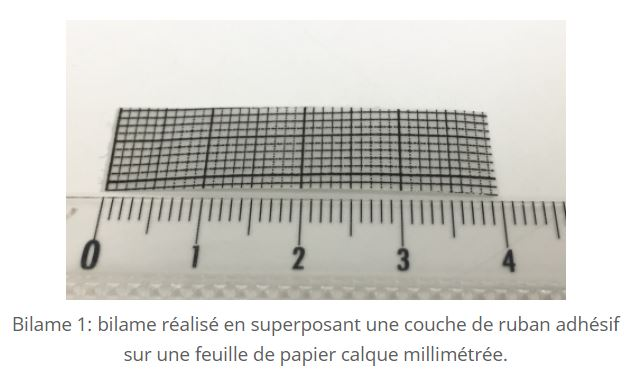
\includegraphics[scale=0.3]{imgs/exp1.JPG}
    \end{figure}
    \begin{figure}
        \centering
        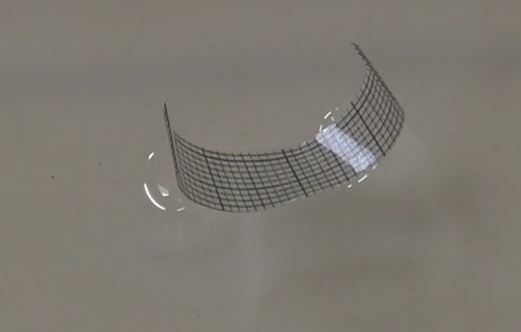
\includegraphics[scale=0.3]{imgs/exp2.JPG}
    \end{figure}
\end{frame}

\begin{frame}{Expérience}
    \begin{figure}
        \centering
        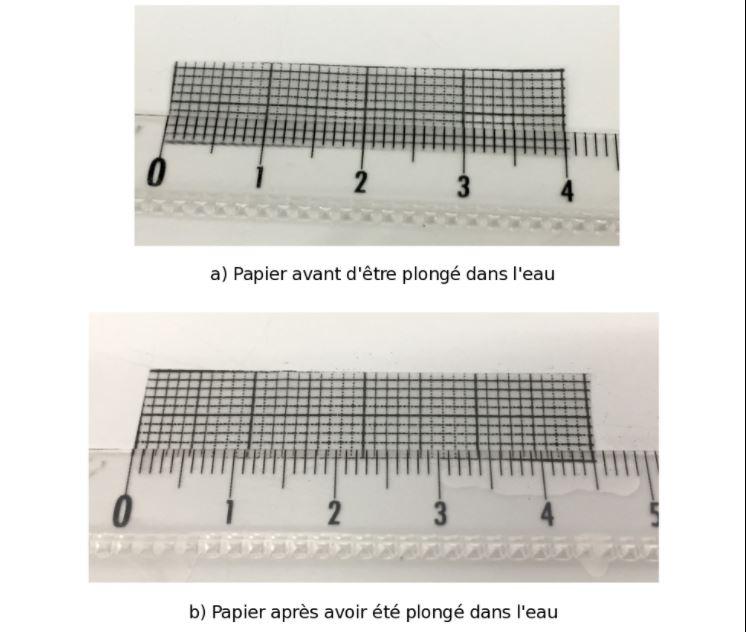
\includegraphics[scale=0.3]{imgs/exp3.JPG}
    \end{figure}
    \begin{itemize}
        \item On constate que le papier s'est dilaté dans l'eau. Par contre, la taille du ruban adhésif reste la même. La dilatation d'un des côtés du bilame provoque une déformation de celui-ci.
    \end{itemize}
    
\end{frame}
